\documentclass{standalone}
\usepackage{tkz-fct}
\usepackage{tkz-euclide}
\usepackage{color}
\renewcommand*\familydefault{\sfdefault}
\usepackage{sansmath}
\usepackage{amsmath}
\sansmath
\definecolor{gray75}{gray}{0.75}
\begin{document}
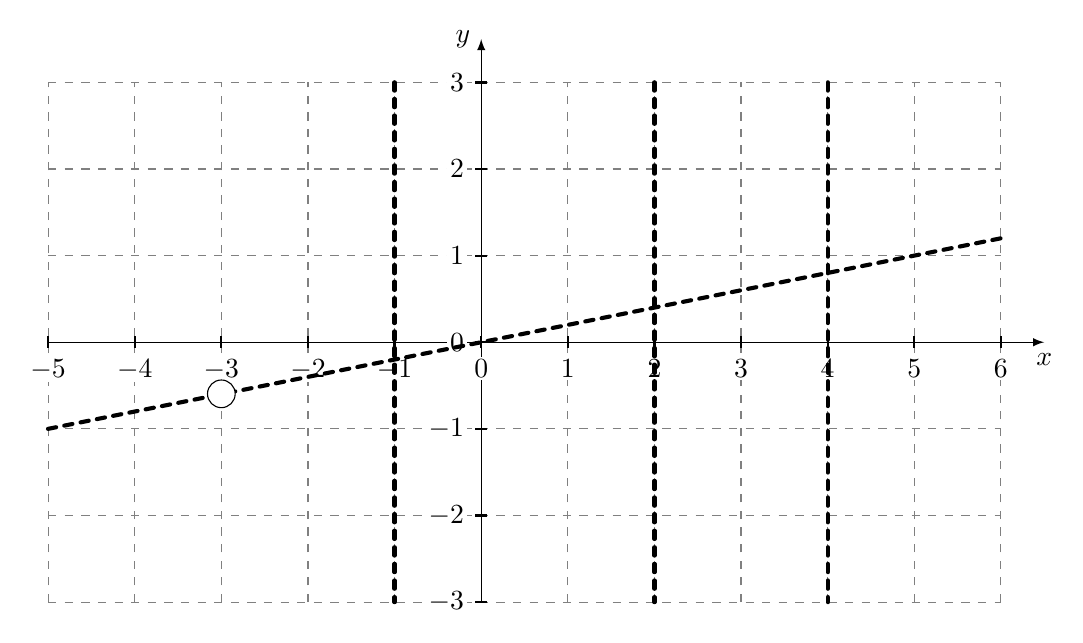
\begin{tikzpicture}[scale=1.1]
  \tkzInit[xmin=-5, xmax=6,ymin=-3,ymax=3]
  \begin{scope}[dashed]
    \tkzGrid
  \end{scope}
  \tkzDrawX[label={$x$}]
  \tkzDrawY[label={$y$}]
  \tkzLabelX
  \tkzLabelY
  \tkzFct[line
  width=2pt,domain=-9:-1.01]{0.2*x+(x**2+3*x)/((x+3)*(x+1)**2*(x-2)**2*(x-4))}
  \tkzFct[line
  width=2pt,domain=-0.95:1.9]{0.2*x+(x**2+3*x)/((x+3)*(x+1)**2*(x-2)**2*(x-4))}
  \tkzFct[line
  width=2pt,domain=2.05:3.99]{0.2*x+(x**2+3*x)/((x+3)*(x+1)**2*(x-2)**2*(x-4))}
  \tkzFct[line
  width=2pt,domain=4.01:9]{0.2*x+(x**2+3*x)/((x+3)*(x+1)**2*(x-2)**2*(x-4))}



  \tkzDefPoint(-1.0,3.0){A}
  \tkzDefPoint(-1.0,-3.0){B}
  \tkzDrawSegment[style=dashed,line width = 1.5pt](A,B)
  \tkzDefPoint(2.0,3.0){A}
  \tkzDefPoint(2.0,-3.0){B}
  \tkzDrawSegment[style=dashed,line width = 1.5pt](A,B)
  \tkzDefPoint(4.0,3.0){A}
  \tkzDefPoint(4.0,-3.0){B}
  \tkzDrawSegment[style=dashed,line width = 1.5pt](A,B)
  \tkzDefPoint(-5.0,-1){A}
  \tkzDefPoint(6.0,1.2){B}
  \tkzDrawSegment[style=dashed,line width = 1.5pt](A,B)
  \tkzDrawPoint[size=10,color=black,fill=white](-3.0,-0.59571)

\end{tikzpicture}
\end{document}
